\documentclass[addpoints]{exam}

%These tell TeX which packages to use.
\usepackage{array,epsfig}
\usepackage{amsmath}
\usepackage{amsfonts}
\usepackage{amssymb}
\usepackage{amsxtra}
\usepackage{amsthm}
\usepackage{../mlextra} % must be below ams packages
\usepackage{mathrsfs}
\usepackage{color}
\usepackage{array}
\usepackage{graphicx}
\graphicspath{ {../../art/} }
\usepackage{bm}
\usepackage{tikz}
\usepackage{multicol}

%Pagination stuff.
\setlength{\topmargin}{-.3 in}
\setlength{\oddsidemargin}{0in}
\setlength{\evensidemargin}{0in}
\setlength{\textheight}{9.in}
\setlength{\textwidth}{6.5in}



\newcommand{\twonode}{%
  \begingroup\normalfont
  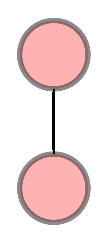
\includegraphics[height=\fontcharht\font`\b]{2nodetree.eps}%
  \endgroup
}


\begin{document}


\noindent
\begin{tabular*}{\textwidth}{l @{\extracolsep{\fill}} r @{\extracolsep{6pt}} l}
{\large CS3001: Foundations of Computer Science} &  \makebox[3in]{\large Name:\enspace\hrulefill}\\
{\large April 22, 2019} & \\
{\large Quiz 2} & 
\end{tabular*}\\

\fbox{\fbox{\parbox{6in}{\textbf{Instructions}: Please answer the questions 
  below to the best of your ability. Be sure to show your work where appropriate. 
   This quiz is closed book, closed notes, closed computer. There are \numpoints\ 
   points in total. }}}\\
\begin{questions}
\question[3] Define the set of strings $K = \{a^{3k} \mid k \in \Z^+ \}$.  
Give a Post system for $K$.

\vspace{30mm}

\question Consider the following Post system for strings over $\Sigma = \{b\}$:

\begin{tabbing}
{\bf R2}XX \=  \kill
{\bf B1} \>
        \(\begin{array}[t]{l}
        bbbbb \in P
        \end{array}\) \\[2ex]
{\bf B2} \>
        \(\begin{array}[t]{l}
        bb \in P
        \end{array}\) \\[2ex]
{\bf R} \>
        \(\begin{array}[t]{l}
        x \in P \;\;\;y \in P \\
        \hline
        xy \in P
        \end{array}\) 
\end{tabbing}

\begin{parts}
\part[2] Prove that $bbbbbbbbb$ (i.e., $b^{9}$) is in $P$. (Hint: a derivation is sufficient).
\vspace{30mm}

\part[3] Consider the set $L = \left \{x \in \Sigma^* \mid \lvert x \rvert \geq 4 \right\}$. Suppose you
were asked to prove that all elements of $L$ are contained in $P$. Which of the following induction rules
should you use:

\begin{tabbing}
[a]XX \=  \kill
[a] \>
	\(\begin{array}[t]{l}
	S(i) \;\wedge\; \forall n \geq i.\;S(i)\;\wedge\;S(i+1)\;\wedge\cdots\wedge\;S(n) \Rightarrow S(n+1) \\
	\hline
	\forall n \geq i. \; S(n)
	\end{array}\)
\end{tabbing}

\begin{tabbing}
[b]XX \=  \kill
[b] \>
	\(\begin{array}[t]{l}
	S(i) \;\wedge\; \forall n \leq i.\;S(i)\;\wedge\;S(i-1)\;\wedge\cdots\wedge\;S(n) \Rightarrow S(n-1) \\
	\hline
	\forall n \leq i. \; S(n)
	\end{array}\)
\end{tabbing}


\begin{tabbing}
[c]XX \=  \kill
[c] \>
	\(\begin{array}[t]{l}
	S(i) \;\wedge\; S(i+1)\;\wedge\cdots\wedge\;S(j)\;\wedge\; \\
\forall n \geq j.\;S(i)\;\wedge\;S(i+1)\;\wedge\cdots\wedge\;S(n) \Rightarrow S(n+1) \\
	\hline
	\forall n \geq i. \; S(n)
	\end{array}\) % \\[2ex]
\end{tabbing}

\begin{tabbing}
[d]XX \=  \kill
[d] \>
	\(\begin{array}[t]{l}
	S(i) \;\wedge\; \forall n \geq i.\;S(n) \Rightarrow S(n+1) \\
	\hline
	\forall n \geq i. \; S(n)
	\end{array}\) % \\[2ex]
\end{tabbing}
~\\Briefly justify your answer:
\end{parts}




\vspace{25mm}
\clearpage



\vspace{25mm}



\vspace{25mm}

\question[3] 
Recall our mutually recursive definition of rooted trees.
\begin{tabbing}
{\bf R2}XX \=  \kill
{\bf B} \>
        \(\begin{array}[t]{l}
        \id{nil}\in\id{RTL}
        \end{array}\) \\[2ex]
{\bf R1} \>
        \(\begin{array}[t]{l}
        t\in\id{RT}\;\;\;l\in\id{RTL} \\
        \hline
        \id{cons}(t,l)\in\id{RTL}
        \end{array}\) \\[2ex]
{\bf R2} \>
        \(\begin{array}[t]{l}
        l\in\id{RTL} \\
        \hline
        \id{node}(l)\in\id{RT}
        \end{array}\)
\end{tabbing}

Given this definition, draw the object described in the derivation below: 

\begin{tabular}{llllllll}
           &                                 &            &                                 & $\bid{B}$  & $\id{nil}\in\id{RTL}$                                                                \\ \cline{6-6}
           &                                 & $\bid{B}$  & $\id{nil}\in\id{RTL}$           & $\bid{R2}$ & $\id{node}(\id{nil})\in\id{RT}$ & $\id{nil}\in\id{RTL}$                  & $\bid{B}$ \\ \cline{4-4} \cline{6-7}
$\bid{B}$  & $\id{nil}\in\id{RTL}$           & $\bid{R2}$ & $\id{node}(\id{nil})\in\id{RT}$ & $\bid{R1}$ & \multicolumn{2}{l}{$\id{cons}(\id{node}(\id{nil}),\id{nil})\in\id{RTL}$}             \\ \cline{2-2} \cline{4-7}
$\bid{R2}$ & $\id{node}(\id{nil})\in\id{RT}$ & $\bid{R1}$ & \multicolumn{3}{l}{$\id{cons}(\id{node}(\id{nil}), \id{cons}(\id{node}(\id{nil}),\id{nil}))\in\id{RTL}$}                            \\ \cline{2-6}
$\bid{R1}$ & \multicolumn{5}{l}{$\id{cons}(\id{node}(\id{nil}), \id{cons}(\id{node}(\id{nil}), \id{cons}(\id{node}(\id{nil}),\id{nil}))) \in \id{RTL}$}                                         \\ \cline{2-6}
$\bid{R2}$ & \multicolumn{5}{l}{$\id{node}(\id{cons}(\id{node}(\id{nil}), \id{cons}(\id{node}(\id{nil}), \id{cons}(\id{node}(\id{nil}),\id{nil}))))\in\id{RT}$}                      
\end{tabular}

%\newpage

\end{questions}
\end{document}


